\documentclass{report}

\input{preamble}
\input{macros}
\input{letterfonts}

\usepackage[dvipsnames]{xcolor}
\usepackage{tikz}
\usetikzlibrary{positioning}
\usepackage{pgfplots}
\usepackage{amsmath}
\usepackage{mathrsfs}

\begin{document}
\noindent\textbf{\huge{Recitation Session}}\hfill Hunter Ellis \\ 
\noindent\textbf{\large{Continuous \& Discrete}}\hfill\today \\
\noindent\rule{\linewidth}{0.4pt}\\

\noindent\textbf{\large{Signals Review}}

\qs{Fourier Transform}{
    For the following time-domain function: \\

\begin{center}
\begin{tikzpicture}
    \begin{axis}[
        axis lines = middle,
        xlabel = $t$,
        ylabel = {$f(t)$},
        ymin = -0.1, ymax = 1.2,
        xmin = -3, xmax = 3,
        xtick = {-1, 1},
        xticklabels = {$-T$, $T$},
        ytick = {0, 1},
        width = 10cm,
        height = 6cm,
        samples = 100
    ]
    \addplot[domain=-3:-1, samples=2, thick, blue] {0};
    \addplot[domain=-1:1, samples=2, thick, blue] {1};
    \addplot[domain=1:3, samples=2, thick, blue] {0};
    
    % Dashed vertical lines
    \addplot[dashed, thick, blue] coordinates {(-1, 0) (-1, 1)};
    \addplot[dashed, thick, blue] coordinates {(1, 0) (1, 1)};
    
    \end{axis}
\end{tikzpicture}
\end{center}

Determine the Fourier Transform, $F(\omega)$, of the the signal (symbolically with $T$).
}
\sol{
    $$
    f(t)=
    \begin{cases}
        1 & -T \leq t \leq T \\
        0 & \text{otherwise}
    \end{cases}
    $$
    \begin{eqnarray*}
        F(\omega)&=&\frac{e^{-j\omega T}-e^{j\omega T}}{-j\omega} \\
                 &=& \frac{2\sin(\omega T)}{\omega}
    \end{eqnarray*}
}
\newpage

\noindent\textbf{\large{Routh-Hurwitz Criterion}}

\noindent Consider a strictly proper transfer function of form:

$$H(s)=\frac{Y(s)}{U(s)}$$

\noindent We would like to determine if the system is strictly stable (i.e. all roots have a real positive component).\\

\noindent Given the denominator polynomial of the $n^{th}$-degree polynomial
$$U(s)=a_{n}s^{n}+a_{n-1}s^{n-1}+a_{n-2}s^{n-2}+...+a_{1}s+a_{0}$$

\noindent We can construct the following \textbf{Routh array}:

$$
\begin{matrix}[c|ccccc]
    s^{n} & a_{n} & a_{n-2} & a_{n-4} &  ...\\
    s^{n-1} & a_{n-1} & a_{n-3} & a_{n-5} &  ... \\ 
\end{matrix}
$$

\nt{You may pad zeros at the end of the array where necessary}

\noindent We then construct the third row, $s^{n-2}$:

$$
\begin{matrix}[c|ccccc]
    s^{n} & a_{n} & a_{n-2} & a_{n-4} & a_{n-6} & ...\\
    s^{n-1} & a_{n-1} & a_{n-3} & a_{n-5} & a_{n-7} & ... \\ 
    s^{n-2} & b_{1} & b_{2} & b_{3} & b_{4} & ... \\ 
\end{matrix}
$$

\noindent Where $b$'s are a determined by the formula,

$$b_{1}=-\frac{\text{det}
\begin{vmatrix}
    a_{n} & a_{n-2} \\
    a_{n-1} & a_{n-3}
\end{vmatrix}}{a_{n-1}}
,\ 
b_{2}=-\frac{\text{det}
\begin{vmatrix}
    a_{n} & a_{n-4} \\
    a_{n-1} & a_{n-5}
\end{vmatrix}}{a_{n-1}}
,\ 
b_{3}=-\frac{\text{det}
\begin{vmatrix}
    a_{n} & a_{n-6} \\
    a_{n-1} & a_{n-7}
\end{vmatrix}}{a_{n-1}}
,\ ...
$$

\noindent We continue this process for the following rows:

$$
\begin{matrix}[c|ccccc]
    s^{n} & a_{n} & a_{n-2} & a_{n-4} & a_{n-6} & ...\\
    s^{n-1} & a_{n-1} & a_{n-3} & a_{n-5} & a_{n-7} & ... \\ 
    s^{n-2} & b_{1} & b_{2} & b_{3} & b_{4} & ... \\ 
    s^{n-3} & c_{1} & c_{2} & c_{3} & c_{4} & ... \\ 
\end{matrix}
$$

$$
c_{1}=-\frac{\text{det}
\begin{vmatrix}
    a_{n-1} & a_{n-3} \\
    b_{1} & b_{2}
\end{vmatrix}}{b_{1}}
,\ 
c_{2}=-\frac{\text{det}
\begin{vmatrix}
    a_{n-1} & a_{n-5} \\
    b_{1} & b_{3}
\end{vmatrix}}{b_{1}}
,\ 
c_{3}=-\frac{\text{det}
\begin{vmatrix}
    a_{n-1} & a_{n-7} \\
    b_{1} & b_{4}
\end{vmatrix}}{b_{1}}
,\ ...
$$

\noindent Util row $s_{0}$ is reached.

\thm{The Routh-Hurwitz Criterion}{
The number of sign changes in the first column of the Routh Table is equal to the number of roots in the right hand plane.
}

\noindent We can use this to determine the stability of the system. 

\newpage

\qs{Routh-Hurwitz Criterion}{
    Determine if the system is stable. If not, how many poles are in the right half-plane.
    $$\frac{s+15}{s^{3}+10s^{2}+31s+1030}$$

}
\sol{
$$
\begin{matrix}[c|ccccc]
    s^{3} & 1 & 31 & 0 \\
    s^{2} & 10 & 1030 & 0 \\ 
    s^{1} & -72 & 0 & 0 \\ 
    s^{0} & 103 & 0 & 0 \\ 
\end{matrix}
$$
There are two sign changes 10$\rightarrow$-72 and -72$\rightarrow$103, thus two poles in the right plane.
}
\newpage

\noindent\textbf{\large{Laplace, Complex Analysis, and Applications}}

\qs{Laplace Transform}{
    Find the Laplace Transform of the following function:
    $$f(t)=t^{2}e^{-3t},\ t\geq 0$$
}
\sol{
$$
\mathcal{L}\{t^{2}e^{-3t}\} = \frac{2}{(s+3)^{3}},\ s>-3
$$
}\newpage

\qs{Cauchy-Riemann}{
    Verify whether the following function $f(z)$ given $z=x+jy$ is differentiable over all points $\mathbb{C}$.
$$
f(z)=z^{2}
$$
}
\sol{
    $$
    \frac{\partial u}{\partial x} = \frac{\partial v}{\partial y} = 2x
    $$
    $$
    \frac{\partial u}{\partial y} = -\frac{\partial v}{\partial x} = -2y
    $$

}\newpage

\qs{Inital Value Problem with Laplace}{
    Find $y(t)$ from the following differential equation using Laplace transform,
    $$2\ddot{y}-10\dot{y}+9y=5t$$
    Given the inital conditions, $y(0)=0$ and $\dot{y}(0)=-2$
}
\sol{
    $$y(t)=\frac{1}{125}(-96e^{\frac{t}{2}}+96e^{-2t}-10te^{-2t}-\frac{25}{2}t^{2}e^{-2t})$$
}\newpage

\qs{Bode Plot}{
Create an approximate bode plot for the following transfer function:
    $$H(s)=\frac{500(s+1)}{(s+5)(s+10)}$$
}
\sol{\\
\begin{center}
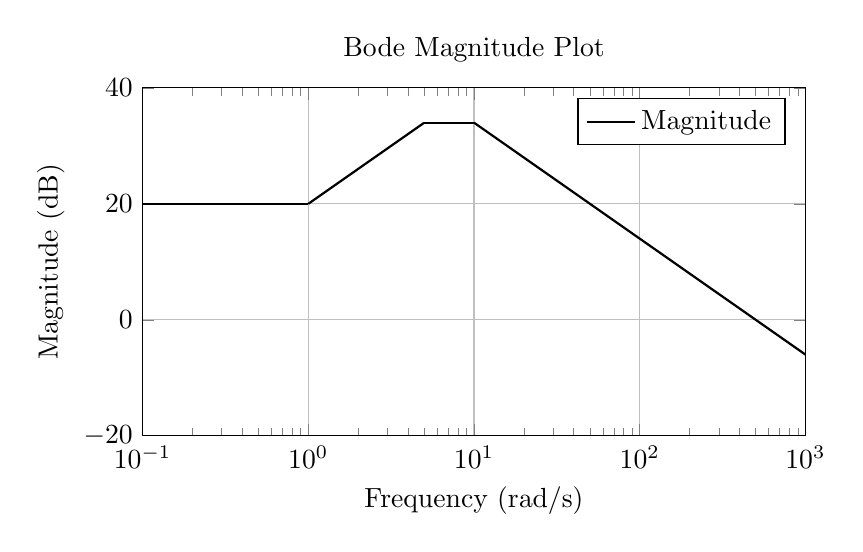
\begin{tikzpicture}
    \begin{semilogxaxis}[
        title={Bode Magnitude Plot},
        xlabel={Frequency (rad/s)},
        ylabel={Magnitude (dB)},
        grid=major,
        width=10cm,
        height=6cm,
        xmin=0.1, xmax=1000,
        ymin=-20, ymax=40,
        xtick={0.1,1,10,100,1000},
        ytick={-40,-20,0,20,40},
        legend pos=north east
    ]
    % Magnitude plot
    \addplot[domain=0.1:1, samples=100, thick] {20};
    \addplot[domain=1:5, samples=100, thick] {20+20*log10(x)};
    \addplot[domain=5:10, samples=100, thick] {34};
    \addplot[domain=10:1000, samples=100, thick] {34 - 20*log10(x/10)};
    \legend{Magnitude}
    \end{semilogxaxis}
\end{tikzpicture}

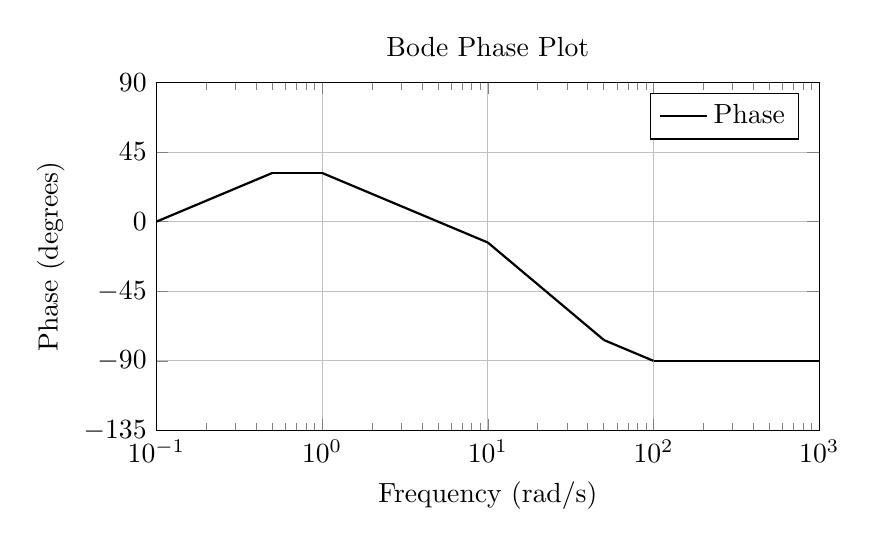
\begin{tikzpicture}
    \begin{semilogxaxis}[
        title={Bode Phase Plot},
        xlabel={Frequency (rad/s)},
        ylabel={Phase (degrees)},
        grid=major,
        width=10cm,
        height=6cm,
        xmin=0.1, xmax=1000,
        ymin=-135, ymax=90,
        xtick={0.1,1,10,100,1000},
        ytick={-135,-90,-45,0,45,90},
        legend pos=north east
    ]
    % Phase plot
    \addplot[domain=0.1:0.5, samples=100, thick] {45*log10(x*10)};
    \addplot[domain=0.5:1, samples=100, thick] {31.5};
    \addplot[domain=1:10, samples=100, thick] {31.5-45*log10(x)};
    \addplot[domain=10:50, samples=100, thick] {-13.5-90*log10(x/10)};
    \addplot[domain=50:100, samples=100, thick] {-76.5-45*log10(x/50)};
    \addplot[domain=100:1000, samples=100, thick] {-90)};
    \legend{Phase}
    \end{semilogxaxis}
\end{tikzpicture}
\end{center}
}\newpage

\end{document}
